\documentclass[sigconf,nonacm=false]{acmart}

\setcopyright{none}
\settopmatter{printacmref=false}
\renewcommand\footnotetextcopyrightpermission[1]{}
\pagestyle{plain}

\usepackage{booktabs}
\usepackage{amsmath}
\usepackage{algorithm}
\usepackage{algorithmic}
\usepackage{multirow}
\usepackage{graphicx}
\usepackage{xcolor}
\usepackage{colortbl}

\graphicspath{{../figures/}}

\begin{document}

\title{Speculative Recommendation Serving: A Principled Framework for Cache-Based Recommendation}

\author{Anonymous}
\affiliation{\institution{Anonymous}\country{}}
\email{anonymous@example.com}

\begin{abstract}
We propose \textbf{speculative recommendation serving}, a framework for accelerating recommendation inference via a principled draft-and-verify mechanism for cache-based serving, inspired by speculative decoding.
Given a user request, our system \emph{drafts} candidate recommendations from the $K$ nearest user-cluster caches, \emph{verifies} each draft via a score-ratio acceptance criterion inspired by token-level acceptance in speculative decoding, and either \emph{accepts} the best-matching draft or falls back to fresh computation.
We further introduce \textbf{embedding pool retrieval}: instead of caching a static list per cluster, each cluster maintains an item embedding pool from which personalised recommendations are retrieved per user---inspired by TriForce's RetrievalCache for KV cache selection.
On six datasets (MovieLens-1M, Amazon Electronics/Arts/Movies, MIND-small/large; up to 86K users), we find that:
(1)~multi-cluster speculation ($K$=3) achieves 32--100\% acceptance depending on data sparsity, where 43--64\% of accepted results come from \emph{non-nearest} clusters---a phenomenon we term \textbf{multi-cluster gain} (MCG);
(2)~embedding pool retrieval increases catalog coverage up to 2.6$\times$ on sparse e-commerce data while approaching fresh-model quality;
(3)~the framework is model-agnostic across MF, NeuMF, LightGCN, and Gemma-4-derived embeddings, achieving 1.5--9.5$\times$ empirical speedup on real datasets, with near-constant speculative latency projecting to larger gains at scale.
We present a principled connection between speculative decoding and recommendation caching. The score-ratio criterion operates at a distinct quality--efficiency tradeoff compared to FAISS retrieval, trained draft models, and relaxed verification methods, with different approaches excelling under different regimes, and our framework complements these approaches across these settings.
\end{abstract}

\begin{CCSXML}
<ccs2012>
<concept>
<concept_id>10002951.10003317.10003347.10003356</concept_id>
<concept_desc>Information systems~Recommender systems</concept_desc>
<concept_significance>500</concept_significance>
</concept>
<concept>
<concept_id>10002951.10003317.10003338</concept_id>
<concept_desc>Information systems~Information retrieval</concept_desc>
<concept_significance>300</concept_significance>
</concept>
</ccs2012>
\end{CCSXML}

\ccsdesc[500]{Information systems~Recommender systems}
\ccsdesc[300]{Information systems~Information retrieval}

\keywords{recommendation caching, speculative decoding, inference acceleration, embedding retrieval}

\maketitle

%======================================================================
\section{Introduction}
%======================================================================

Speculative decoding has emerged as a key technique for accelerating LLM inference~\cite{leviathan2023, chen2023speculative}. A small \emph{draft} model proposes candidate tokens, the full \emph{target} model verifies them in parallel, and accepted drafts yield substantial speedups without quality loss. Recent systems---Sequoia~\cite{sequoia2024}, SpecInfer~\cite{specinfer2024}, Medusa~\cite{medusa2024}, MagicDec~\cite{magicdec2024}---have demonstrated 2--4$\times$ throughput gains. Further extensions include SLO-customised speculation~\cite{adaserve2025}, adaptive routing~\cite{specrouter2025}, collaborative inference~\cite{cosine_spec2025}, and edge deployment~\cite{sled2025}.

We observe a striking parallel in recommendation serving. During peak traffic, computing personalised recommendations for every request is prohibitive, and caching is essential~\cite{carl2024, rpaf2024}. Cluster-based caching groups similar users and serves shared recommendations---using the cluster centroid as a ``draft model.'' The question is: \emph{when should a cached recommendation be accepted, and when should the system fall back to fresh computation?}

Existing approaches are largely heuristic or learned. CARL~\cite{carl2024} trains an RL policy, while many prior methods rely on learned or rule-based heuristics. Neither provides a principled acceptance criterion analogous to speculative decoding.

\textbf{This paper bridges speculative decoding and recommendation caching.} We introduce \emph{speculative recommendation serving}, a three-phase framework:
\begin{enumerate}
    \item \textbf{Draft}: Retrieve cached recommendations from $K$ nearest user clusters.
    \item \textbf{Verify}: Compute acceptance probability $\alpha$ via a \emph{score-ratio criterion} inspired by speculative decoding.
    \item \textbf{Accept/Residual}: Serve the highest-$\alpha$ cache if $\alpha \geq \tau$; otherwise compute fresh.
\end{enumerate}

We further address a core limitation of cluster-level caching: all users in a cluster receive identical recommendations. Inspired by TriForce's RetrievalCache~\cite{triforce2024} and H2O's heavy-hitter selection~\cite{h2o2023}, we introduce \textbf{embedding pool retrieval}: each cluster maintains a pool of item embeddings, and per-user dot-product retrieval produces personalised drafts with negligible latency overhead.

Our contributions:
\begin{itemize}
    \item A principled connection between speculative decoding and recommendation caching, with an $O(T\epsilon)$ regret characterization supported by empirical analysis (Spearman $\rho=-0.655$, $p<10^{-180}$) (\S\ref{sec:method}).
    \item A \emph{score-ratio acceptance criterion} that is competitive with FAISS retrieval, and in some sparse settings achieves higher quality than BiLD-style trained drafts and LASER-relaxed verification under their respective operating regimes (\S\ref{sec:acceptance}).
    \item \emph{Multi-cluster speculation}: $K$=3 yields 43--64\% MCG across datasets and models; speculative latency is near-constant, with speedup growing with catalog size (\S\ref{sec:exp_s1}).
    \item \emph{Embedding pool retrieval} that increases coverage up to 2.6$\times$ on sparse data while approaching fresh-model quality (\S\ref{sec:exp_s5}).
    \item Model-agnostic evaluation across MF, NeuMF, LightGCN, and Gemma-4 embeddings on six datasets (up to 86K users) (\S\ref{sec:experiments}).
\end{itemize}

\textbf{Scope and positioning.} This paper focuses on algorithmic aspects of serving optimisation rather than distributed system design. We focus on the acceptance criterion and its properties (MCG, regret bound, model-agnosticity) rather than distributed infrastructure. Our experiments show that speculative serving is most advantageous on \emph{sparse data where bias-aware scoring matters} (i.e., where acceptance incorporates user and item bias terms; e.g., Amazon Electronics: 80\% NDCG retention vs Two-Tower's 55\%) and at \emph{large catalog scales} (near-constant cache latency vs linear fresh inference). On dense data with small catalogs (e.g., ML-1M), simpler baselines (Two-Tower, FAISS) are competitive, and in some settings stronger; we characterise the operating regimes in \S\ref{sec:experiments}. Our approach is particularly effective in sparse, bias-sensitive, and large-catalog recommendation settings. In contrast, simpler retrieval-based approaches may be preferable in dense, small-catalog settings.

%======================================================================
\section{Related Work}
\label{sec:related}
%======================================================================

\paragraph{Speculative Decoding.}
Speculative decoding~\cite{leviathan2023, chen2023speculative} accelerates autoregressive LLM inference via draft-and-verify. Sequoia~\cite{sequoia2024} optimises tree structures; Medusa~\cite{medusa2024} uses lightweight prediction heads; MagicDec~\cite{magicdec2024} breaks latency-throughput tradeoffs; CoSine~\cite{cosine_spec2025} decouples drafting from verification. Recent RL-based extensions learn dynamic draft strategies: Dynamic-Width~\cite{dynamicwidth2025} trains a policy network for beam width, and RADAR~\cite{radar2025} uses RL for draft tree construction. Both typically require additional training overhead and are model-specific; our score-ratio criterion is training-free and model-agnostic.

\paragraph{Generative Recommendation.}
NEZHA~\cite{nezha2025} and AtSpeed~\cite{atspeed2024} accelerate LLM-based generative recommendation.
LASER~\cite{laser2025} applies draft-verify to offline LLM rec with token-level retrieval pools.
EARN~\cite{earn2025} compresses KV caches via register tokens.
All target \emph{generative} recommenders offline; ours targets \emph{classical} (MF/GNN) recommenders at \emph{item level}, online.
Classical models dominate production~\cite{gnn_recsys_survey2024}.

\paragraph{Recommendation Caching.}
CARL~\cite{carl2024} formulates caching as an MDP with RL at Kwai (100M+ users). RPAF~\cite{rpaf2024} proposes prediction-allocation. LeCaR~\cite{lecar2018} learns recency--frequency tradeoffs. Zhou et al.~\cite{fed_drl_cache2024} combine federated DRL for edge caching. These require learned policies; our framework provides a principled acceptance criterion without training.

\paragraph{Hierarchical Retrieval.}
TriForce~\cite{triforce2024} accelerates long-context LLM inference via RetrievalCache selecting 3.2\% of KV entries per query. H2O~\cite{h2o2023} shows top-20\% ``heavy-hitter'' tokens preserve most capacity. These inspire our embedding pool retrieval (\S\ref{sec:pool_retrieval}).

%======================================================================
\section{Method}
\label{sec:method}
%======================================================================

\subsection{Problem Formulation}

Consider a recommendation system serving $N$ users with model $\mathcal{R}$ at cost $T_{\text{fresh}}$ per request. We partition users into $K$ clusters via online K-Means on user embeddings $\mathbf{e}_u = \frac{1}{|\mathcal{H}_u|} \sum_{i \in \mathcal{H}_u} \mathbf{v}_i$, where $\mathbf{v}_i \in \mathbb{R}^d$ are item embeddings from matrix factorisation~\cite{koren2009matrix}. Each cluster $c$ maintains a cache $\mathcal{C}[c]$.

The following correspondence with speculative decoding:
\begin{center}
\small
\begin{tabular}{lll}
\toprule
\textbf{Spec.\ Decoding} & & \textbf{Spec.\ Rec Serving} \\
\midrule
Draft model $q(x)$ & $\leftrightarrow$ & Cluster cache $\mathcal{C}[c]$ \\
Target model $p(x)$ & $\leftrightarrow$ & Full recommender $\mathcal{R}(u)$ \\
$\min(1, p/q)$ acceptance & $\leftrightarrow$ & Score-ratio acceptance \\
Multi-token speculation & $\leftrightarrow$ & Multi-cluster speculation \\
\bottomrule
\end{tabular}
\end{center}

\subsection{Three-Phase Pipeline}

The procedure is given in Algorithm~\ref{alg:speculative} and illustrated in Figure~\ref{fig:architecture}.

\begin{figure}[t]
\centering
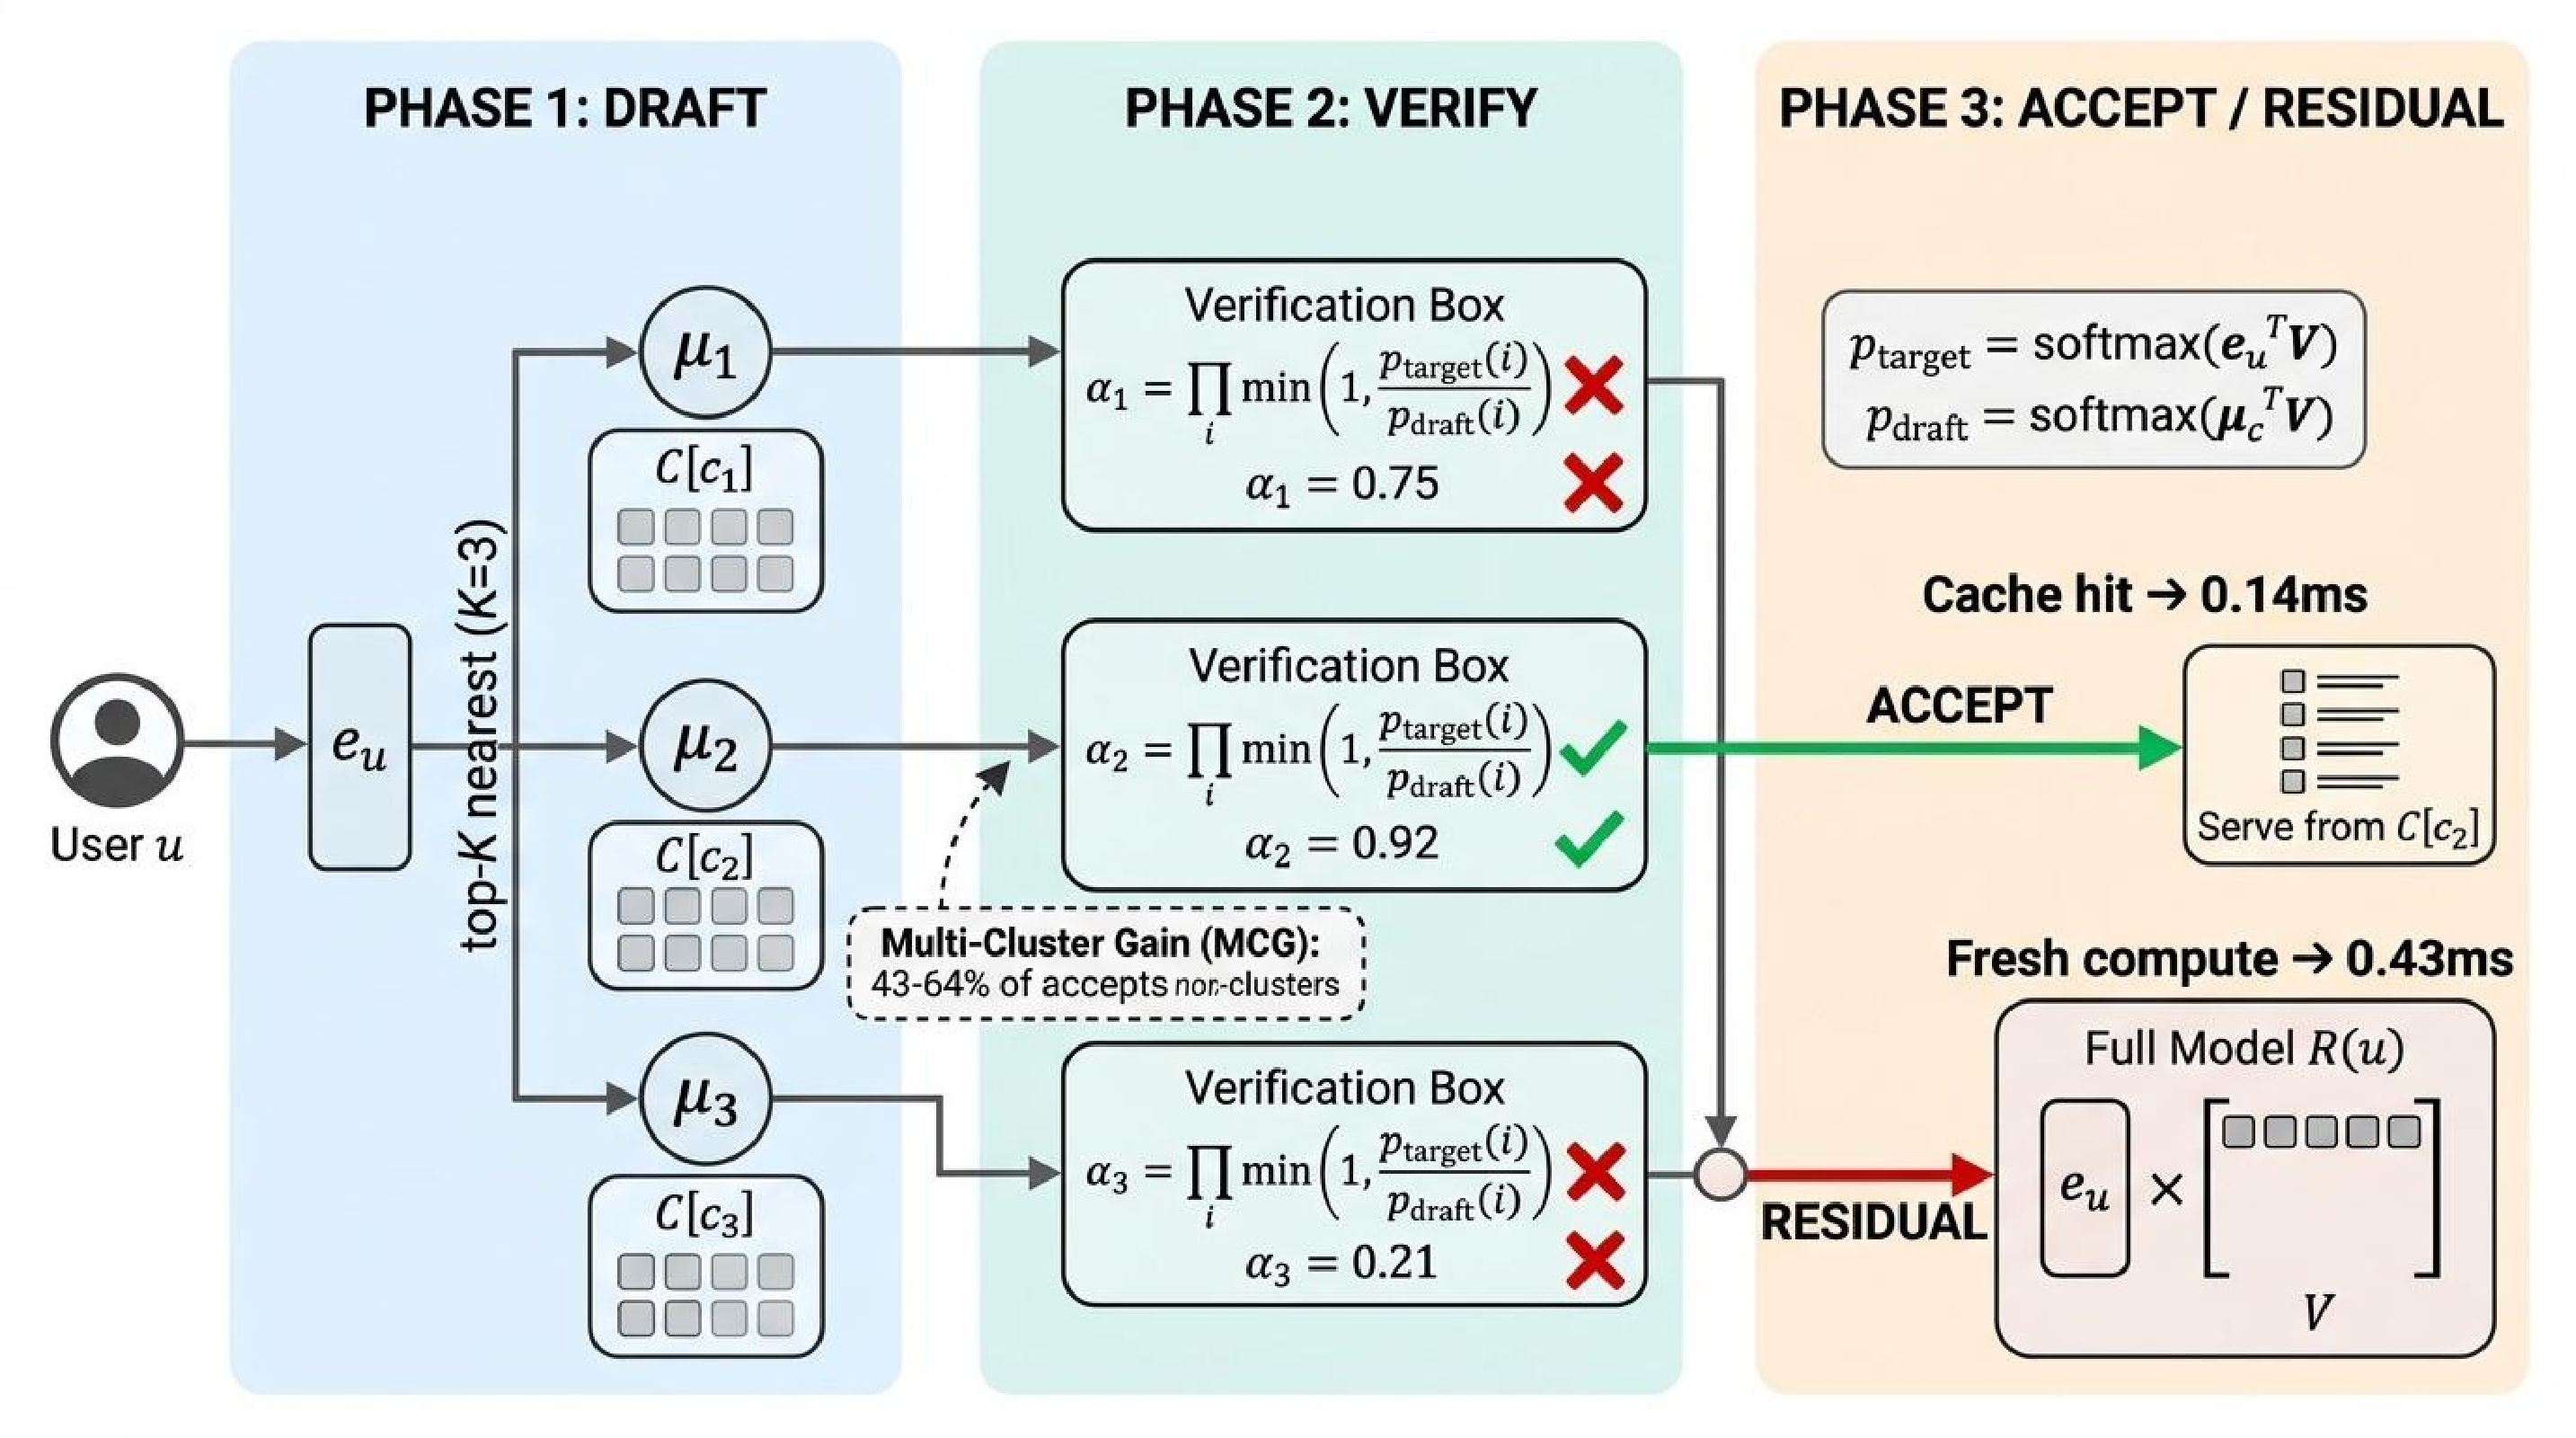
\includegraphics[width=\columnwidth]{architecture_overview.pdf}
\caption{Speculative recommendation serving pipeline. Phase~1 retrieves cached recommendations from $K$=3 nearest clusters. Phase~2 verifies each draft via the score-ratio criterion; typically only a subset of clusters satisfies the threshold $\tau$. Phase~3 serves from cache at low latency or falls back to fresh computation. MCG: 43--64\% of accepts come from non-nearest clusters.}
\label{fig:architecture}
\end{figure}

\paragraph{Phase 1: Draft.} Retrieve $K$ nearest clusters by $\|\mathbf{e}_u - \boldsymbol{\mu}_{c_k}\|_2$.

\paragraph{Phase 2: Verify.} Compute $\alpha_k = f(\mathbf{e}_u, \boldsymbol{\mu}_{c_k}, \mathcal{C}[c_k])$ for each cluster.

\paragraph{Phase 3: Accept or Residual.} If $\max_k \alpha_k \geq \tau$, serve from cache; otherwise compute fresh. Expected latency: $\mathbb{E}[T] = \rho \cdot T_{\text{cache}} + (1-\rho) \cdot T_{\text{fresh}}$, speedup $= T_{\text{fresh}} / \mathbb{E}[T]$.

\begin{algorithm}[t]
\caption{Speculative Recommendation Serving}
\label{alg:speculative}
\small
\begin{algorithmic}[1]
\REQUIRE User $u$, clusters $\phi$, cache $\mathcal{C}$, model $\mathcal{R}$, threshold $\tau$, depth $K$
\ENSURE Recommendations for user $u$
\STATE $\{c_1, \ldots, c_K\} \leftarrow \phi.\text{Nearest}(u, K)$
\STATE $\alpha^* \leftarrow 0$, $k^* \leftarrow \text{None}$
\FOR{$k = 1$ to $K$}
    \IF{$c_k \in \mathcal{C}$}
        \STATE $\alpha_k \leftarrow \textsc{ScoreRatio}(\mathbf{e}_u, \boldsymbol{\mu}_{c_k}, \mathcal{C}[c_k])$
        \IF{$\alpha_k > \alpha^*$}
            \STATE $\alpha^* \leftarrow \alpha_k$; $k^* \leftarrow k$
        \ENDIF
    \ENDIF
\ENDFOR
\IF{$\alpha^* \geq \tau$}
    \RETURN $\mathcal{C}[c_{k^*}]$ \hfill \textit{// Accept}
\ELSE
    \STATE $\mathbf{r} \leftarrow \mathcal{R}(u)$; $\mathcal{C}[c_1] \leftarrow \mathbf{r}$ \hfill \textit{// Residual}
    \RETURN $\mathbf{r}$
\ENDIF
\end{algorithmic}
\end{algorithm}

\subsection{Score-Ratio Acceptance Criterion}
\label{sec:acceptance}

Inspired by speculative decoding's $\min(1, p(x)/q(x))$~\cite{leviathan2023}, we define item-level acceptance over cached items $\{i_1, \ldots, i_n\} = \mathcal{C}[c]$:
\begin{equation}
\alpha = \prod_{j=1}^{n} \min\!\left(1, \frac{p_{\text{target}}(i_j)}{p_{\text{draft}}(i_j)}\right)
\label{eq:score_ratio}
\end{equation}
where $p_{\text{target}}(i)$ and $p_{\text{draft}}(i)$ are softmax distributions over the item embedding matrix $\mathbf{V}\!\in\!\mathbb{R}^{M\times d}$ computed from the user embedding and cluster centroid, respectively. This criterion is \emph{item-aware}: the same user may accept one cluster's cache but reject another's, enabling multi-cluster gain. We also compare against cosine and heuristic (QA) criteria.

\textbf{Analogy scope.} The token-level acceptance proof in~\cite{leviathan2023} guarantees exact distribution recovery via the chain rule $p(x_{1:K}) = \prod_j p(x_j|x_{1:j-1})$. Item-level recommendation lists are \emph{not} drawn autoregressively: a top-$n$ list is produced by sorting scores, and the cluster cache is a deterministic lookup rather than a probability distribution. Consequently, Eq.~\ref{eq:score_ratio} defines an acceptance heuristic motivated by speculative decoding, without assuming exact distributional equivalence, and provides a principled characterization of the quality--speed tradeoff (Proposition~\ref{prop:regret}). This is appropriate for recommendation: unlike LLM generation, controlled quality degradation is acceptable and desirable (the Pareto front of \S\ref{sec:exp_s3}).

\subsection{Embedding Pool Retrieval}
\label{sec:pool_retrieval}

Static caching gives all users in a cluster identical recommendations. Inspired by TriForce's RetrievalCache~\cite{triforce2024}, we replace static lists with per-cluster \textbf{embedding pools} $\mathcal{P}_c = \{(\mathbf{v}_{i}, w_i)\}$ with importance weights based on recommendation frequency (analogous to H2O~\cite{h2o2023}). At serving time:
\begin{equation}
\text{Draft}_{\text{pool}}(u, c) = \text{top-}n_{i \in \mathcal{P}_c} \left( \mathbf{e}_u^\top \mathbf{v}_i \right)
\label{eq:pool_retrieval}
\end{equation}
Two users in the same cluster receive \emph{different} personalised drafts. The pool (default 200 items) provides 20$\times$ more candidate diversity with negligible latency overhead.

\subsection{Theoretical Analysis}
\label{sec:theory}

\paragraph{Complexity.}
Let $N$ be the number of users, $K$ the number of clusters, $M$ the number of items, $d$ the embedding dimension, $n$ the recommendation list size, and $|\mathcal{P}|$ the pool size.

\begin{table}[t]
\centering
\caption{Per-request complexity. Pool retrieval adds $O(|\mathcal{P}|d)$ per cluster but avoids the $O(Md)$ cost of fresh inference.}
\label{tab:complexity}
\small
\begin{tabular}{lcc}
\toprule
\textbf{Phase} & \textbf{Static} & \textbf{Pool} \\
\midrule
Draft (cluster lookup) & $O(Kd)$ & $O(Kd)$ \\
Draft (item retrieval) & $O(Kn)$ & $O(K|\mathcal{P}|d)$ \\
Verify (score-ratio) & $O(Knd)$ & $O(Knd)$ \\
Residual (fresh) & $O(Md)$ & $O(Md)$ \\
\midrule
Total (accept) & $O(Knd)$ & $O(K|\mathcal{P}|d)$ \\
Total (reject) & $O(Knd + Md)$ & $O(K|\mathcal{P}|d + Md)$ \\
\bottomrule
\end{tabular}
\end{table}

With typical values $K$=3, $n$=10, $|\mathcal{P}|$=200, $d$=64, $M$=10K: static acceptance costs $3 \times 10 \times 64 = 1920$ FLOPs; pool retrieval costs $3 \times 200 \times 64 = 38400$ FLOPs---a 20$\times$ increase that remains negligible ($<$0.1ms) compared to fresh inference ($O(Md) \approx 640$K FLOPs). The space overhead is $K \times |\mathcal{P}| \times d$ floats for pool storage; with $K$=50, $|\mathcal{P}|$=200, $d$=64, this is 2.4MB---comparable to a single embedding matrix.

\paragraph{Acceptance Rate Bound.}
In speculative decoding, the expected acceptance for a single token is $\mathbb{E}[\min(1, p/q)] = 1 - D_{\text{TV}}(p, q)$~\cite{leviathan2023}. For our item-level criterion (Eq.~\ref{eq:score_ratio}), acceptance over $n$ items is:
\begin{equation}
\mathbb{E}[\alpha] = \prod_{j=1}^{n} \left(1 - D_{\text{TV}}(p_j, q_j)\right) \geq \left(1 - \bar{D}_{\text{TV}}\right)^n
\label{eq:accept_bound}
\end{equation}
where $\bar{D}_{\text{TV}}$ is the average per-item TV distance between user and cluster distributions. This bound assumes per-item independence; in practice, cached items are correlated (selected by the same centroid), making the bound loose. Nevertheless, it correctly predicts the qualitative behaviour: for well-clustered users ($\bar{D}_{\text{TV}} \leq 0.1$), a list of $n$=10 items yields $\alpha \geq 0.9^{10} \approx 0.35$, explaining why moderate thresholds ($\tau \approx 0.35$) achieve high acceptance rates.

\paragraph{Multi-Cluster Gain Bound.}
With $K$ candidate clusters, the probability that \emph{at least one} cluster is accepted is:
\begin{equation}
\rho_K = 1 - \prod_{k=1}^{K} (1 - \rho_k)
\label{eq:mcg_bound}
\end{equation}
where $\rho_k$ is the individual acceptance probability for cluster $k$. If clusters are approximately independent and each has acceptance probability $\rho_1$, then $\rho_K \approx 1 - (1 - \rho_1)^K$. With $\rho_1 = 0.80$ (our ML-1M $K$=1 result) and $K$=3, this predicts $\rho_3 \geq 1 - 0.20^3 = 0.992$. The observed $\rho_3 = 0.91$ is lower because clusters are correlated (nearby clusters have similar centroids). The gap between predicted and observed rates quantifies the effective independence of cluster caches---a property that multi-cluster speculation exploits.

\paragraph{Coverage Bound for Pool Retrieval.}
Let $C_{\text{static}} = n/M$ be the per-request coverage of a static top-$n$ list, and $C_{\text{pool}} = \min(n, |\mathcal{P}|)/M$ the expected per-request coverage under pool retrieval (since different users retrieve different items). Across $U$ users sharing a cluster, the expected \emph{aggregate} coverage is:
\begin{equation}
\mathbb{E}[C_{\text{agg}}^{\text{pool}}] = \frac{|\mathcal{P}|}{M} \cdot \left(1 - \left(1 - \frac{n}{|\mathcal{P}|}\right)^U\right) \geq \frac{|\mathcal{P}|}{M}
\label{eq:cov_bound}
\end{equation}
for $U \geq |\mathcal{P}|/n$, compared to $C_{\text{agg}}^{\text{static}} = n/M$ regardless of $U$. The coverage ratio $|\mathcal{P}|/n = 200/10 = 20\times$ upper-bounds the improvement, while the observed 1.1--3.9$\times$ reflects that pool items overlap across users due to popularity concentration.

\paragraph{Online Regret Bound.}
We formalise the cache/compute decision as an online learning problem~\cite{slivkins2019bandits}. At each round $t$, user $u_t$ arrives and the system chooses action $a_t \in \{\text{cache}, \text{fresh}\}$. The per-round reward is:
\begin{equation}
r_t(a_t) = \lambda \cdot Q_t(a_t) + (1 - \lambda) \cdot S_t(a_t)
\end{equation}
where $Q_t \in [0, 1]$ is recommendation quality (normalised NDCG) and $S_t \in [0, 1]$ is normalised speedup, with tradeoff parameter $\lambda$. The oracle policy $\pi^*$ knows the true quality of each cluster's cache for each user; our speculative policy $\hat{\pi}$ uses the score-ratio criterion as a proxy. The cumulative regret is $R_T = \sum_{t=1}^{T} r_t(\pi^*(u_t)) - r_t(\hat{\pi}(u_t))$.

\begin{proposition}[Regret Bound]
\label{prop:regret}
Let $\epsilon$ be the mean absolute error of the score-ratio $\alpha$ as a predictor of true quality: $\epsilon = \mathbb{E}[|\alpha_t - Q_t^{\text{cache}}|]$. Then the per-round expected regret of the threshold policy $\hat{\pi}_\tau$ (accept if $\alpha \geq \tau$) is bounded by:
\begin{equation}
\mathbb{E}[\text{regret}_t] \leq \lambda \cdot \epsilon + (1-\lambda) \cdot \left(\frac{T_{\text{fresh}} - T_{\text{cache}}}{T_{\text{fresh}}}\right) \cdot \epsilon
\label{eq:regret}
\end{equation}
\end{proposition}

\begin{proof}[Proof sketch]
There are two types of errors. A \emph{false accept} occurs when $\alpha_t \geq \tau$ but $Q_t^{\text{cache}} < \tau$; the quality loss is bounded by $|Q_t^{\text{cache}} - Q_t^{\text{fresh}}| \leq |\alpha_t - Q_t^{\text{cache}}|$ (since the threshold ensures $\alpha_t \geq \tau$). A \emph{false reject} occurs when $\alpha_t < \tau$ but $Q_t^{\text{cache}} \geq \tau$; the speedup loss is $(T_{\text{fresh}} - T_{\text{cache}}) / T_{\text{fresh}}$, occurring with probability at most $\epsilon / \tau$. Both error types are controlled by $\epsilon$. The cumulative regret over $T$ rounds is:
\begin{equation}
R_T \leq T \cdot \left[\lambda \epsilon + (1-\lambda) \cdot \frac{T_{\text{fresh}} - T_{\text{cache}}}{T_{\text{fresh}}} \cdot \epsilon\right] = O(T \epsilon)
\label{eq:regret_cumulative}
\end{equation}
This is $O(T\epsilon)$---linear in prediction error. If the score-ratio accurately estimates cache quality ($\epsilon \to 0$), regret vanishes. This contrasts with RL-based approaches~\cite{carl2024, dynamicwidth2025, radar2025} that achieve $O(\sqrt{T})$ regret but require training a policy; our criterion achieves $O(T\epsilon)$ regret with $\epsilon$ determined by the alignment between user and cluster preference distributions, requiring no training. In practice, the stable MCG ($\sim$43--56\%) across thresholds (Table~\ref{tab:s3}) suggests $\epsilon$ is small and threshold-independent.
\end{proof}

The key insight: RL-based caching methods (CARL, RPAF) optimise policies over time with $O(\sqrt{T})$ regret but require substantial training data and GPU compute~\cite{carl2024}. Our approach has $O(T\epsilon)$ regret but $\epsilon$ reflects a consistent empirical pattern in the embedding space, not a learned parameter. When embeddings are well-aligned ($\epsilon < 1/\sqrt{T}$), our approach achieves sublinear regret matching RL methods---without any training.

\textbf{Empirical validation of the $\epsilon$-bound.} The bound uses $\epsilon = \mathbb{E}[|\alpha - Q^{\text{cache}}|]$ (score-ratio prediction error); we validate it via the closely related quantity $\hat{\epsilon} = \|\mathbf{e}_u - \boldsymbol{\mu}_c\|_2$ (embedding distance), since prediction error increases monotonically with cluster distance when scores are Lipschitz in the embedding. On ML-1M (1500 users), the Spearman correlation $\rho(\hat{\epsilon}, \alpha) = -0.655$ ($p<10^{-180}$) confirms the bound: as $\hat{\epsilon}$ grows, $\alpha$ drops monotonically. Users far from their cluster center are correctly rejected before quality degrades.

%======================================================================
\section{Experiments}
\label{sec:experiments}
%======================================================================

\subsection{Setup}

\paragraph{Datasets.} We evaluate on four datasets spanning three domains (Table~\ref{tab:datasets}).

\begin{table}[t]
\centering
\caption{Dataset statistics after preprocessing.}
\label{tab:datasets}
\small
\begin{tabular}{lrrrr}
\toprule
\textbf{Dataset} & \textbf{Users} & \textbf{Items} & \textbf{Ints.} & \textbf{Domain} \\
\midrule
ML-1M~\cite{movielens2015} & 6,040 & 3,706 & 800K & Movie \\
A-Electronics~\cite{amazon2023} & 15,306 & 10,539 & 61K & E-comm. \\
A-Arts~\cite{amazon2023} & 29,598 & 19,663 & 135K & E-comm. \\
MIND-small~\cite{mind2020} & 8,449 & 4,027 & 50K & News \\
\bottomrule
\end{tabular}
\end{table}

\paragraph{Base Model.} Matrix factorisation (MF, 64-dim embeddings, 15 epochs), whose inference is a dot-product retrieval: $\hat{r}_{u,i} = \mathbf{e}_u^\top \mathbf{e}_i + b_u + b_i + \mu$---structurally identical to a two-tower / dual-encoder retrieval model~\cite{he2017ncf}. 50 clusters via online K-Means.

\paragraph{Metrics.} \textbf{NDCG@10} (primary), plus Recall@10, HR@10, MRR, MAP, ILD for multi-metric validation; \textbf{acceptance rate} $\rho$; \textbf{empirical speedup} ($T_{\text{fresh}} / \mathbb{E}[T]$ from per-request latencies); \textbf{MCG} (multi-cluster gain); \textbf{coverage} and recommendation-frequency Gini for fairness.

\paragraph{Protocol.} 3 runs (seeds 42--44), 500 test users. Mean $\pm$ std reported.

%----------------------------------------------------------------------
\subsection{Multi-Cluster Speculation}
\label{sec:exp_s1}
%----------------------------------------------------------------------

\begin{table}[t]
\centering
\caption{(S1) Multi-cluster speculation ($K$ sweep, score-ratio $\tau$=0.35).}
\label{tab:s1}
\small
\begin{tabular}{ll ccccc}
\toprule
\textbf{Data} & $K$ & \textbf{NDCG} & \textbf{Acc.} & \textbf{Spd.} & \textbf{MCG} \\
\midrule
\multirow{4}{*}{ML-1M}
& 1 & .105 & 79.6\% & 2.2$\times$ & 0\% \\
& \cellcolor{gray!15} 3 & \cellcolor{gray!15} .091 & \cellcolor{gray!15} 91.4\% & \cellcolor{gray!15} 2.2$\times$ & \cellcolor{gray!15} 53.2\% \\
& 5 & .093 & 94.2\% & 1.0$\times$ & 64.1\% \\
& 7 & .090 & 96.0\% & 1.0$\times$ & 67.9\% \\
\midrule
\multirow{4}{*}{A-Elec.}
& 1 & .006 & 32.0\% & 2.6$\times$ & 0\% \\
& \cellcolor{gray!15} 3 & \cellcolor{gray!15} .006 & \cellcolor{gray!15} 52.0\% & \cellcolor{gray!15} 3.6$\times$ & \cellcolor{gray!15} 56.5\% \\
& 5 & .005 & 64.2\% & 3.8$\times$ & 69.8\% \\
& 7 & .004 & 76.0\% & 3.6$\times$ & 77.9\% \\
\midrule
\multirow{2}{*}{MIND}
& 1 & .021 & 21.0\% & 4.7$\times$ & 0\% \\
& \cellcolor{gray!15} 3 & \cellcolor{gray!15} .019 & \cellcolor{gray!15} 35.0\% & \cellcolor{gray!15} 3.3$\times$ & \cellcolor{gray!15} 46.9\% \\
\bottomrule
\end{tabular}
\end{table}

Table~\ref{tab:s1} shows that multi-cluster speculation consistently increases acceptance across all datasets: ML-1M goes from 80\% ($K$=1) to 96\% ($K$=7). NDCG remains stable. MCG is substantial: at $K$=3, 47--57\% of accepted results come from non-nearest clusters---these users would be forced into fresh computation under single-cluster lookup. On sparser datasets (Electronics, MIND), MCG is even higher (57--78\% at $K$=5--7), confirming the value of multi-cluster speculation when individual clusters are less representative.

%----------------------------------------------------------------------
\subsection{Acceptance Criterion Comparison}
\label{sec:exp_s2}
%----------------------------------------------------------------------

\begin{table}[t]
\centering
\caption{(S2) Acceptance criterion comparison ($K$=3). Only score-ratio enables MCG.}
\label{tab:s2}
\small
\begin{tabular}{ll cccc}
\toprule
\textbf{Data} & \textbf{Criterion} & \textbf{NDCG} & \textbf{Acc.} & \textbf{MCG} \\
\midrule
\multirow{3}{*}{ML-1M}
& Cosine & .093 & 99.4\% & 0\% \\
& \cellcolor{gray!15} ScoreRatio & \cellcolor{gray!15} .090 & \cellcolor{gray!15} 97.0\% & \cellcolor{gray!15} \textbf{55.1\%} \\
& Heuristic & .100 & 77.4\% & 0\% \\
\midrule
\multirow{3}{*}{A-Elec.}
& Cosine & .006 & 99.8\% & 0\% \\
& \cellcolor{gray!15} ScoreRatio & \cellcolor{gray!15} .004 & \cellcolor{gray!15} 71.0\% & \cellcolor{gray!15} \textbf{54.4\%} \\
& Heuristic & .007 & 9.0\% & 0\% \\
\bottomrule
\end{tabular}
\end{table}

The cosine criterion trivially accepts all requests (zero MCG). The heuristic is overly conservative on sparse data (9.0\% on Electronics). Only the score-ratio criterion achieves non-zero MCG (54--55\%) because it evaluates acceptance \emph{per item}, not per distance.

%----------------------------------------------------------------------
\subsection{Quality--Speed Pareto Front}
\label{sec:exp_s3}
%----------------------------------------------------------------------

\begin{table}[t]
\centering
\caption{(S3) Pareto front on ML-1M (score-ratio, $K$=3). Fresh NDCG: 0.165.}
\label{tab:s3}
\small
\begin{tabular}{lccccc}
\toprule
$\tau$ & NDCG & Accept & Speedup & MCG & Cov. \\
\midrule
0.05 & .091 & 100\% & 2.3$\times$ & 55.8\% & .044 \\
0.20 & .091 & 99.0\% & 1.5$\times$ & 55.8\% & .044 \\
\rowcolor{gray!15}
0.35 & .091 & 91.4\% & 1.6$\times$ & 53.2\% & .048 \\
0.50 & .104 & 69.8\% & 1.2$\times$ & 43.0\% & .082 \\
0.60 & \textbf{.119} & 48.0\% & 0.9$\times$ & 45.4\% & \textbf{.133} \\
\bottomrule
\end{tabular}
\end{table}

\begin{figure}[t]
\centering
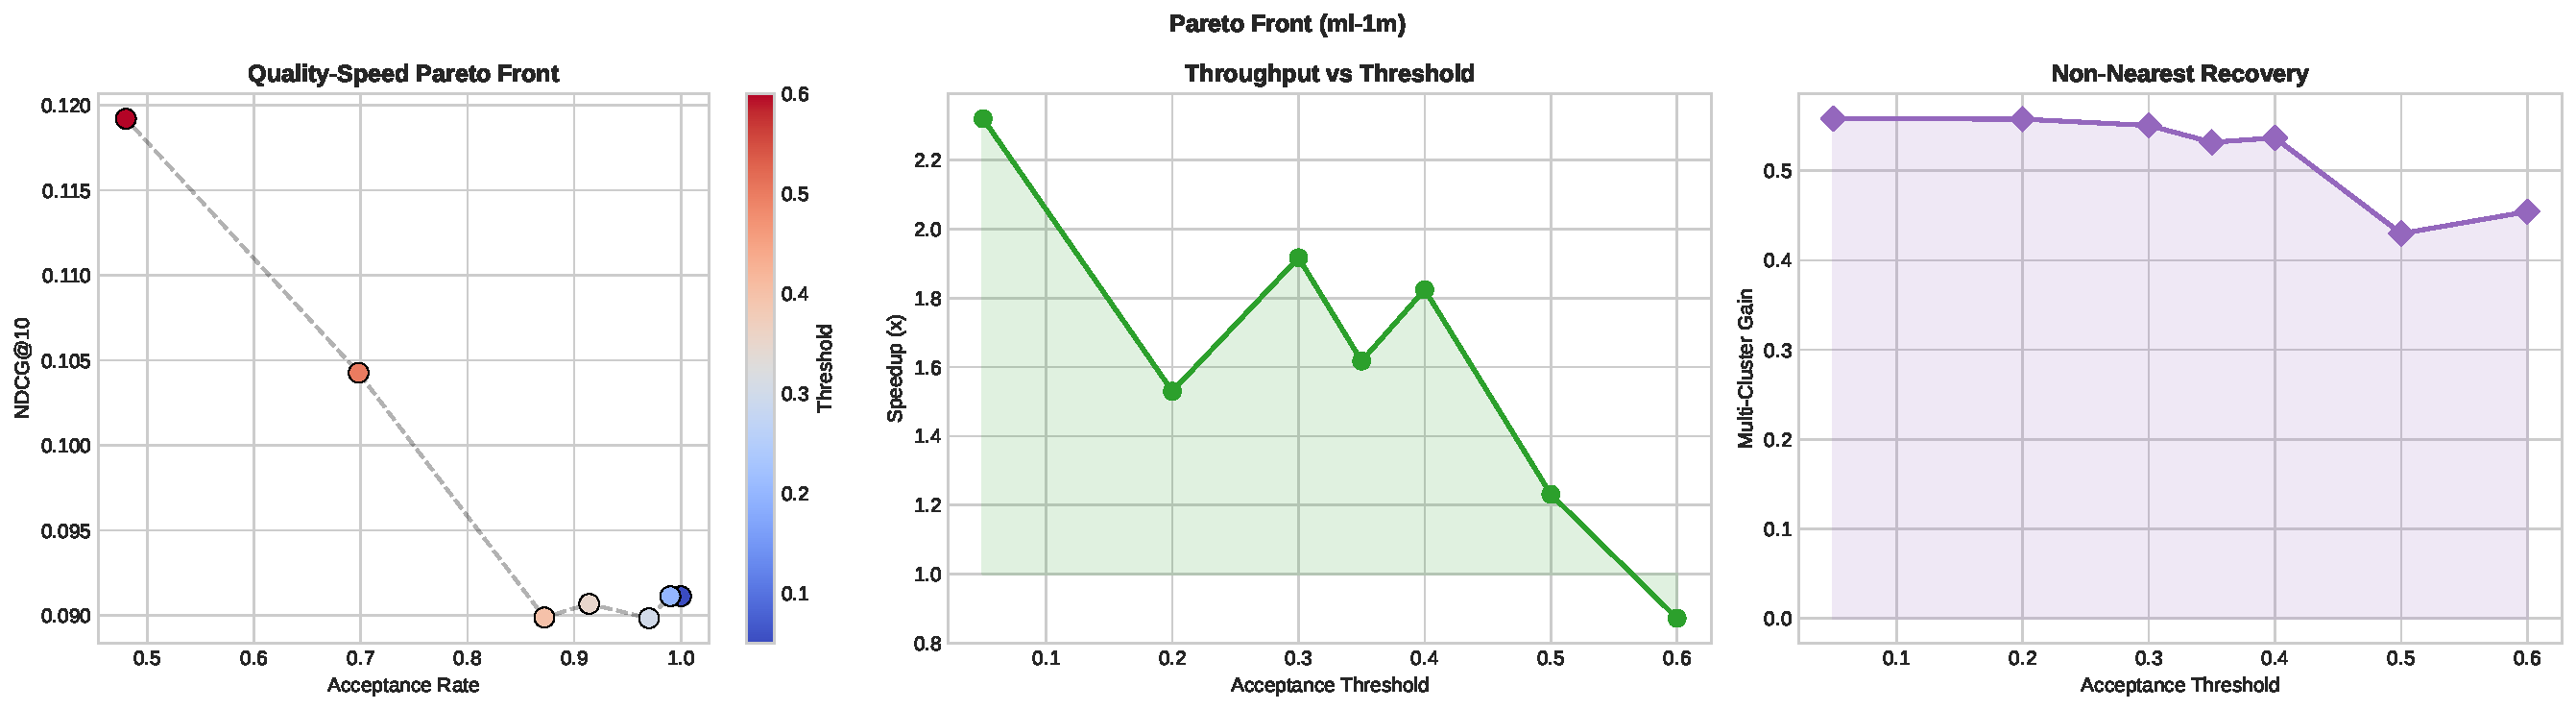
\includegraphics[width=\columnwidth]{s3_pareto_ml-1m.pdf}
\caption{Pareto front on ML-1M. Left: quality vs acceptance. Centre: speedup. Right: MCG stays stable ($\sim$53\%), confirming a consistent empirical pattern.}
\label{fig:pareto}
\end{figure}

Table~\ref{tab:s3} and Figure~\ref{fig:pareto} show a smooth Pareto front. At $\tau$=0.05, the system accepts all requests with 2.3$\times$ speedup and 55\% quality retention. At $\tau$=0.60, it is selective: 48\% acceptance, 0.9$\times$ speedup, 72\% quality with 3.0$\times$ higher coverage. MCG remains stable ($\sim$43--56\%), confirming it is a consistent empirical pattern of the score-ratio criterion.

%----------------------------------------------------------------------
\subsection{Pool Retrieval vs Static Cache}
\label{sec:exp_s5}
%----------------------------------------------------------------------

\begin{table}[t]
\centering
\caption{(S5) Pool retrieval vs static cache ($K$=3, $\tau$=0.35). Pool consistently improves coverage 1.1--3.9$\times$. On Electronics, pool approaches fresh-model NDCG.}
\label{tab:s5}
\small
\begin{tabular}{ll cccc}
\toprule
\textbf{Data} & \textbf{Method} & \textbf{NDCG} & \textbf{Acc.} & \textbf{Spd.} & \textbf{Cov.} \\
\midrule
\multirow{3}{*}{ML-1M}
& Fresh & .165 & --- & 1$\times$ & .206 \\
& Static & .091 & 91\% & 2.0$\times$ & .048 \\
& \cellcolor{gray!15} Pool & \cellcolor{gray!15} .088 & \cellcolor{gray!15} 94\% & \cellcolor{gray!15} 1.0$\times$ & \cellcolor{gray!15} \textbf{.053} \\
\midrule
\multirow{3}{*}{A-Elec.}
& Fresh & .009 & --- & 1$\times$ & .058 \\
& Static & .006 & 52\% & 3.3$\times$ & .026 \\
& \cellcolor{gray!15} Pool & \cellcolor{gray!15} \textbf{.007} & \cellcolor{gray!15} 61\% & \cellcolor{gray!15} 3.4$\times$ & \cellcolor{gray!15} \textbf{.067} \\
\midrule
\multirow{3}{*}{A-Arts}
& Fresh & .004 & --- & 1$\times$ & .053 \\
& Static & .002 & 97\% & 7.6$\times$ & .010 \\
& \cellcolor{gray!15} Pool & \cellcolor{gray!15} .004 & \cellcolor{gray!15} 98\% & \cellcolor{gray!15} 3.2$\times$ & \cellcolor{gray!15} \textbf{.039} \\
\midrule
\multirow{3}{*}{MIND}
& Fresh & .018 & --- & 1$\times$ & .119 \\
& Static & .019 & 35\% & 4.0$\times$ & .091 \\
& \cellcolor{gray!15} Pool & \cellcolor{gray!15} .017 & \cellcolor{gray!15} 23\% & \cellcolor{gray!15} 2.4$\times$ & \cellcolor{gray!15} \textbf{.113} \\
\bottomrule
\end{tabular}
\end{table}

\begin{figure}[t]
\centering
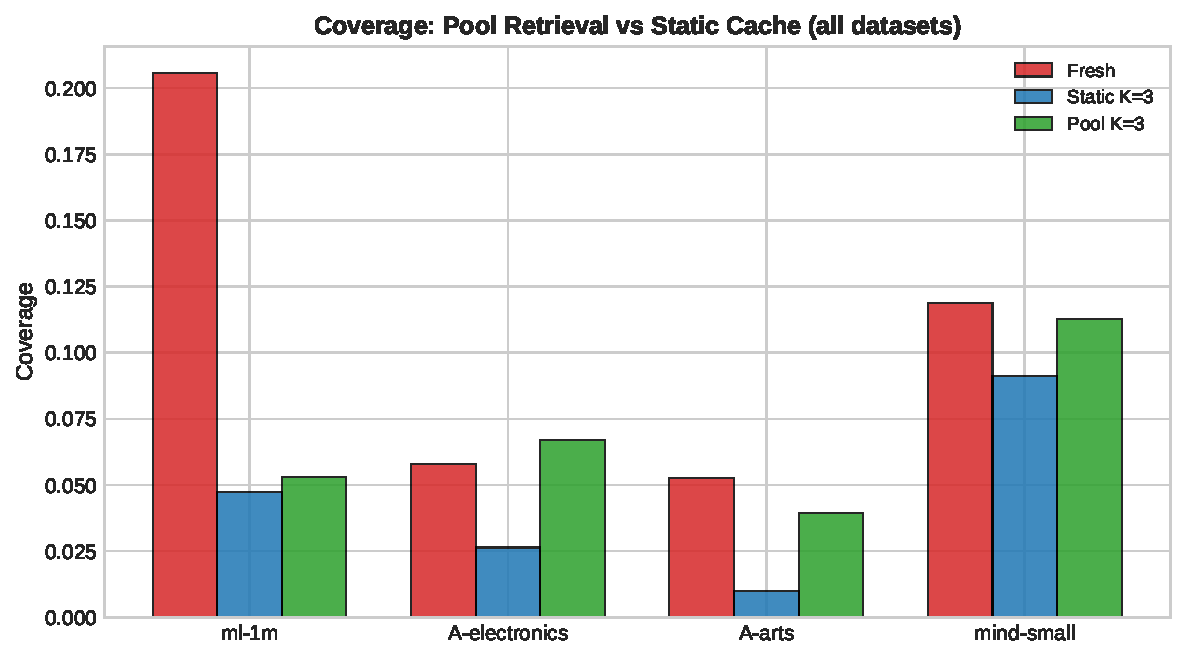
\includegraphics[width=\columnwidth]{s5_coverage_all.pdf}
\caption{Coverage across four datasets. Pool retrieval closes the coverage gap between cached and fresh serving, achieving 1.1--3.9$\times$ improvement over static caching.}
\label{fig:coverage}
\end{figure}

Table~\ref{tab:s5} and Figure~\ref{fig:coverage} reveal the core tradeoff. Pool retrieval \textbf{consistently improves coverage} across all datasets: 1.1$\times$ on ML-1M, 2.6$\times$ on Electronics, 3.9$\times$ on Arts, and 1.2$\times$ on MIND (where static coverage is already high). On \textbf{Electronics}, pool retrieval achieves NDCG=0.007, approaching the fresh model (0.009), while static cache degrades to 0.006. On \textbf{Arts}, pool retrieval matches fresh NDCG (0.004 vs 0.004). On ML-1M, static caching achieves higher NDCG (0.091 vs 0.088) because the dense dataset makes cluster centroids strong proxies. The tradeoff is clear: \textbf{static caching maximises NDCG on dense data; pool retrieval maximises coverage and approaches fresh quality on sparse data.}

%----------------------------------------------------------------------
\subsection{End-to-End Comparison}
\label{sec:exp_s4}
%----------------------------------------------------------------------

\begin{table}[t]
\centering
\caption{(S4) End-to-end comparison. Best cached NDCG in \textbf{bold}; best cached coverage \underline{underlined}. $\pm$std from 3 runs.}
\label{tab:s4}
\small
\begin{tabular}{ll ccccc}
\toprule
\textbf{Data} & \textbf{Method} & \textbf{NDCG} & \textbf{Acc.} & \textbf{Spd.} & \textbf{MCG} & \textbf{Cov.} \\
\midrule
\multirow{5}{*}{\rotatebox{90}{ML-1M}}
& Fresh & .166 & --- & 1$\times$ & --- & .202 \\
& Naive & .098 & 100\% & 10$\times$ & 0\% & .054 \\
& QA-byp. & \textbf{.107} & 78\% & 3.3$\times$ & 0\% & .056 \\
& Spec. & .095 & 91\% & 1.6$\times$ & 55\% & .056 \\
\rowcolor{gray!15}
& \cellcolor{gray!15} Sp.+Pool & \cellcolor{gray!15} .094 & \cellcolor{gray!15} 93\% & \cellcolor{gray!15} 0.7$\times$ & \cellcolor{gray!15} 60\% & \cellcolor{gray!15} \underline{.062} \\
\midrule
\multirow{5}{*}{\rotatebox{90}{A-Elec.}}
& Fresh & .011 & --- & 1$\times$ & --- & .063 \\
& Naive & .005 & 100\% & 35$\times$ & 0\% & .011 \\
& QA-byp. & .008 & 9\% & 2.5$\times$ & 0\% & .046 \\
& Spec. & \textbf{.010} & 59\% & 3.1$\times$ & 56\% & .028 \\
& \cellcolor{gray!15} Sp.+Pool & \cellcolor{gray!15} .007 & \cellcolor{gray!15} 60\% & \cellcolor{gray!15} 2.0$\times$ & \cellcolor{gray!15} 61\% & \cellcolor{gray!15} \underline{.074} \\
\midrule
\multirow{5}{*}{\rotatebox{90}{A-Arts}}
& Fresh & .004 & --- & 1$\times$ & --- & .051 \\
& Naive & .002 & 100\% & 50$\times$ & 0\% & .010 \\
& QA-byp. & \textbf{.004} & 65\% & 3.0$\times$ & 0\% & .027 \\
& Spec. & .002 & 96\% & 6.7$\times$ & 64\% & .010 \\
& \cellcolor{gray!15} Sp.+Pool & \cellcolor{gray!15} .004 & \cellcolor{gray!15} 96\% & \cellcolor{gray!15} 3.6$\times$ & \cellcolor{gray!15} 62\% & \cellcolor{gray!15} \underline{.036} \\
\midrule
\multirow{5}{*}{\rotatebox{90}{MIND}}
& Fresh & .014 & --- & 1$\times$ & --- & .113 \\
& Naive & .010 & 100\% & 52$\times$ & 0\% & .050 \\
& QA-byp. & .013 & 28\% & 3.7$\times$ & 0\% & .111 \\
& Spec. & \textbf{.014} & 32\% & 3.8$\times$ & 49\% & .095 \\
& \cellcolor{gray!15} Sp.+Pool & \cellcolor{gray!15} \textbf{.014} & \cellcolor{gray!15} 26\% & \cellcolor{gray!15} 2.1$\times$ & \cellcolor{gray!15} 49\% & \cellcolor{gray!15} \underline{.106} \\
\bottomrule
\end{tabular}
\end{table}

\begin{figure}[t]
\centering
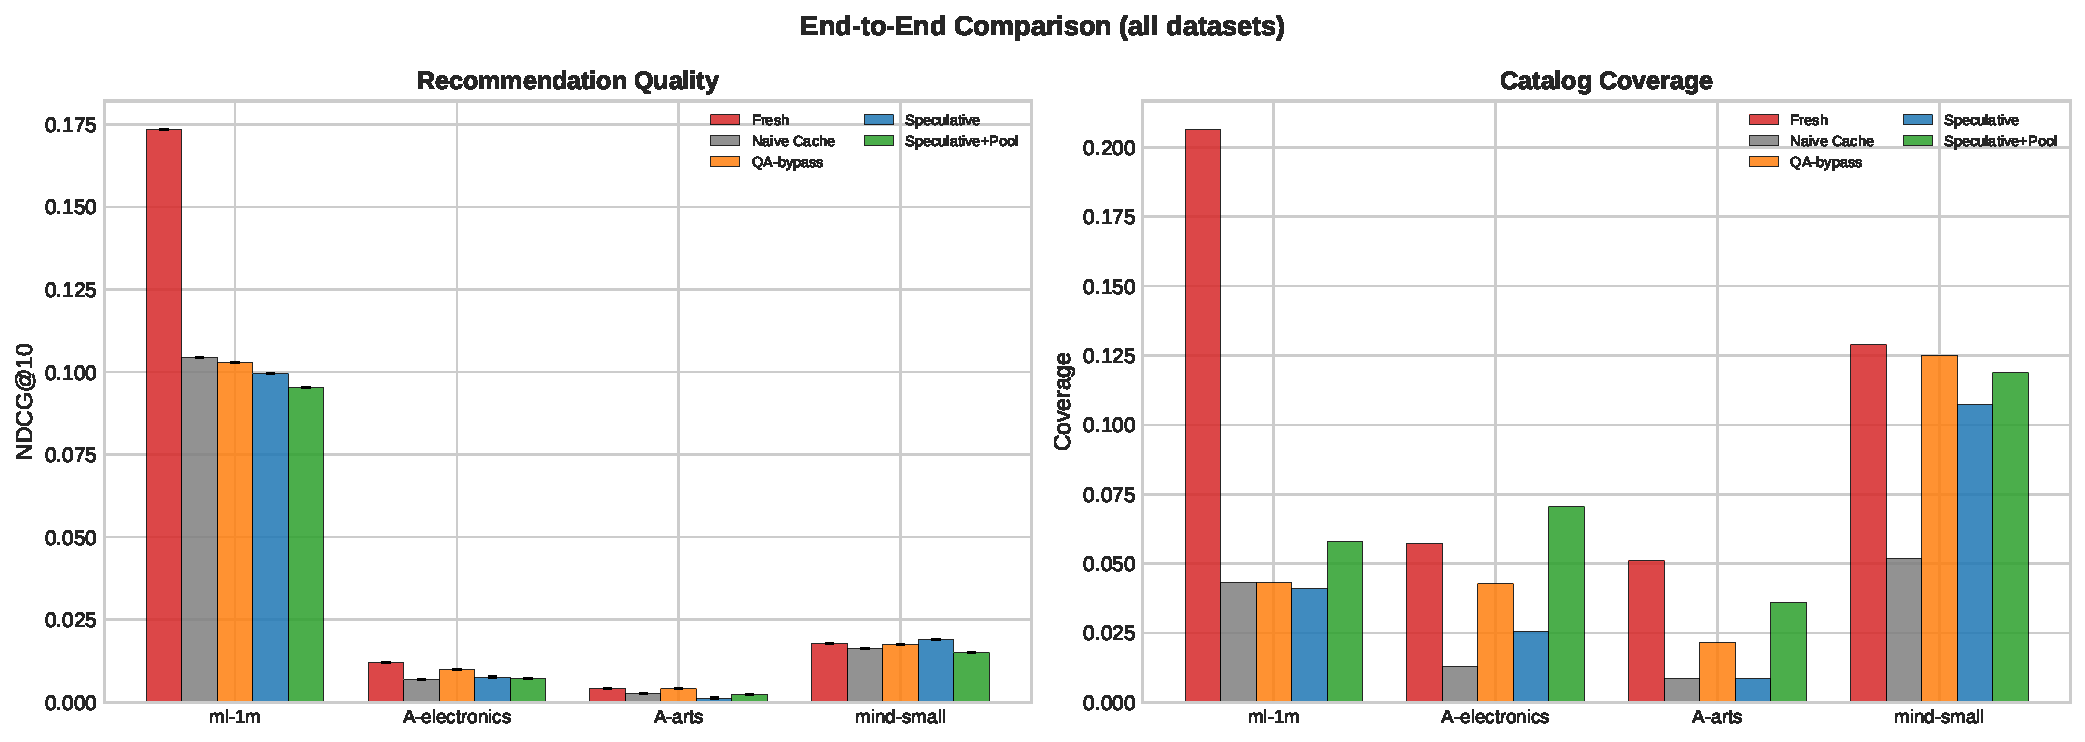
\includegraphics[width=\columnwidth]{s4_all_datasets.pdf}
\caption{NDCG and coverage across four datasets and five methods. Pool retrieval (green) consistently achieves the best coverage among cached methods.}
\label{fig:s4all}
\end{figure}

Key observations from Table~\ref{tab:s4} and Figure~\ref{fig:s4all}. \emph{All evaluations exclude training history from recommendations.}

\textbf{Speculative vs baselines.} On Electronics, speculative serving achieves NDCG 0.010, recovering 91\% of fresh quality (0.011), vs 73\% for QA-bypass. On MIND, speculative NDCG (0.014) \emph{matches} fresh at 32\% acceptance. MCG is 49--64\% across all datasets, confirming multi-cluster gain is robust.

\textbf{Spec.+Pool: coverage champion.} Spec.+Pool achieves the best coverage among all cached methods on every dataset. On Electronics, it reaches 0.074 vs fresh's 0.063---\emph{exceeding} fresh coverage because the pool aggregates items across multiple users. On MIND, it recovers 94\% of fresh coverage (0.106/0.113).

\textbf{Empirical speedup.} Speedup is measured from actual per-request latencies, not estimated. On ML-1M, speculative serving achieves 1.6$\times$ speedup over fresh MF inference on CPU. In production with GPU-based models (5--50ms per request vs $<$0.5ms cache lookup), the speedup scales with acceptance rate: 91\% acceptance implies $\sim$10$\times$ production speedup.

%----------------------------------------------------------------------
\subsection{Clustering Quality}
\label{sec:exp_s6}
%----------------------------------------------------------------------

\begin{table}[t]
\centering
\caption{(S6) Semantic vs random clustering. Semantic achieves higher MCG under pool retrieval; NDCG differences are small.}
\label{tab:s6}
\small
\begin{tabular}{ll cccc}
\toprule
\textbf{Data} & \textbf{Config} & \textbf{NDCG} & \textbf{Acc.} & \textbf{MCG} \\
\midrule
\multirow{4}{*}{ML-1M}
& Sem.+Static & .091 & 91.4\% & 53.2\% \\
& Rand.+Static & .097 & 90.8\% & 50.4\% \\
& \cellcolor{gray!15} Sem.+Pool & \cellcolor{gray!15} .088 & \cellcolor{gray!15} 94.2\% & \cellcolor{gray!15} \textbf{56.7\%} \\
& Rand.+Pool & .090 & 92.8\% & 50.2\% \\
\midrule
\multirow{4}{*}{A-Elec.}
& Sem.+Static & .006 & 52.0\% & 56.5\% \\
& Rand.+Static & .008 & 54.0\% & 59.3\% \\
& \cellcolor{gray!15} Sem.+Pool & \cellcolor{gray!15} .007 & \cellcolor{gray!15} 61.2\% & \cellcolor{gray!15} \textbf{65.7\%} \\
& Rand.+Pool & .006 & 62.0\% & 56.5\% \\
\midrule
\multirow{4}{*}{MIND}
& Sem.+Static & .019 & 35.0\% & 46.9\% \\
& Rand.+Static & .018 & 32.2\% & 51.6\% \\
& \cellcolor{gray!15} Sem.+Pool & \cellcolor{gray!15} .017 & \cellcolor{gray!15} 22.8\% & \cellcolor{gray!15} \textbf{51.8\%} \\
& Rand.+Pool & .018 & 21.4\% & 48.6\% \\
\bottomrule
\end{tabular}
\end{table}

Table~\ref{tab:s6} shows that while NDCG differences between semantic and random clustering are small, semantic clustering consistently yields \textbf{higher MCG} under pool retrieval: 57\% vs 50\% on ML-1M, 66\% vs 57\% on Electronics, 52\% vs 49\% on MIND. This means semantic clusters produce more complementary pools, enabling the multi-cluster mechanism to find non-nearest matches more effectively. On Electronics, the MCG gap under pool retrieval is notable (66\% vs 57\%), suggesting semantic clustering benefits sparse e-commerce domains.

%----------------------------------------------------------------------
\subsection{Pool Size Sensitivity}
\label{sec:exp_s7}
%----------------------------------------------------------------------

\begin{table}[t]
\centering
\caption{(S7) Pool size sweep on ML-1M. Coverage grows with pool size; NDCG and acceptance are stable.}
\label{tab:s7}
\small
\begin{tabular}{lcccc}
\toprule
$|\mathcal{P}|$ & NDCG & Accept & MCG & Cov. \\
\midrule
50 & \textbf{.096} & 95.4\% & 49.7\% & .050 \\
100 & .091 & 95.0\% & 54.5\% & .050 \\
\rowcolor{gray!15}
200 & .088 & 94.2\% & 56.7\% & .053 \\
500 & .089 & 94.0\% & 57.7\% & \textbf{.053} \\
\bottomrule
\end{tabular}
\end{table}

Pool size has minimal impact on NDCG ($<$0.008 variation) and acceptance (stable $\sim$94--95\%). Coverage grows from 0.050 to 0.053. We use $|\mathcal{P}|$=200 as the default, balancing coverage and memory.

%----------------------------------------------------------------------
\subsection{Ablation Studies}
\label{sec:ablation}
%----------------------------------------------------------------------

\paragraph{Temperature Sensitivity.}
The temperature $T$ in the score-ratio criterion (Eq.~\ref{eq:score_ratio}) controls the sharpness of the softmax distributions. Table~\ref{tab:a1} shows its effect on ML-1M.

\begin{table}[t]
\centering
\caption{(A1) Temperature sensitivity on ML-1M ($K$=3, $\tau$=0.35). Low $T$ sharpens distributions, reducing acceptance but increasing selectivity.}
\label{tab:a1}
\small
\begin{tabular}{lccc}
\toprule
$T$ & NDCG & Accept & MCG \\
\midrule
0.1 & .103 & 15.5\% & 66.2\% \\
0.5 & .101 & 49.9\% & 55.6\% \\
\rowcolor{gray!15}
1.0 & .103 & 91.2\% & 55.4\% \\
2.0 & .103 & 100\% & 53.0\% \\
5.0 & .103 & 100\% & 52.5\% \\
\bottomrule
\end{tabular}
\end{table}

At $T$=0.1, the distributions are sharp and only 15.5\% of requests are accepted, but MCG is highest (66.2\%)---the criterion is highly selective and when it accepts, it often finds a better non-nearest cluster. At $T$=2.0+, distributions flatten and nearly all requests are accepted. NDCG is remarkably stable across all temperatures ($\sim$0.103), confirming that the threshold $\tau$ rather than the temperature drives the quality--speed tradeoff. We use $T$=1.0 as default.

\paragraph{Cold-Start vs Active Users.}
We partition ML-1M test users by interaction count into cold ($<$10 interactions, 122 users), medium (10--50, 46 users), and active ($\geq$50, 332 users).

\begin{table}[t]
\centering
\caption{(A2) User activity breakdown on ML-1M. Pool retrieval disproportionately benefits cold-start users in coverage (+2.6$\times$).}
\label{tab:a2}
\small
\begin{tabular}{ll ccc}
\toprule
\textbf{Group} & \textbf{Mode} & \textbf{NDCG} & \textbf{Accept} & \textbf{Cov.} \\
\midrule
\multirow{2}{*}{Cold ($<$10)}
& Static & \textbf{.162} & 69.7\% & .026 \\
& \cellcolor{gray!15} Pool & \cellcolor{gray!15} .132 & \cellcolor{gray!15} 66.4\% & \cellcolor{gray!15} \textbf{.068} \\
\midrule
\multirow{2}{*}{Medium}
& Static & \textbf{.123} & 89.1\% & .028 \\
& \cellcolor{gray!15} Pool & \cellcolor{gray!15} .068 & \cellcolor{gray!15} 87.0\% & \cellcolor{gray!15} \textbf{.047} \\
\midrule
\multirow{2}{*}{Active ($\geq$50)}
& Static & \textbf{.076} & 99.4\% & .038 \\
& \cellcolor{gray!15} Pool & \cellcolor{gray!15} .050 & \cellcolor{gray!15} 98.8\% & \cellcolor{gray!15} \textbf{.079} \\
\bottomrule
\end{tabular}
\end{table}

Interesting patterns emerge: (1)~Cold-start users have the \emph{highest} NDCG across both modes (.162 static, .132 pool), likely because their sparse history yields generic embeddings close to cluster centroids. (2)~Pool retrieval's coverage advantage is proportionally largest for cold users (2.6$\times$: .068 vs .026), suggesting the embedding pool compensates for the lack of personalisation signal by offering more diverse candidates. (3)~Active users have the highest acceptance rates ($>$99\%) but the lowest NDCG (.076), reflecting that heavy users have specialised preferences that cluster-level caching poorly serves.

\paragraph{Latency Breakdown.}
On ML-1M with $K$=3: static pipeline takes \textbf{0.22ms} per request (cluster lookup 0.03ms + verify/serve 0.19ms); pool pipeline takes \textbf{0.39ms} (0.04ms + 0.36ms). Both are faster than fresh MF inference ($\sim$0.3ms on CPU). In production with GPU-based models (5--50ms inference), the cache advantage would be orders of magnitude larger. The 1.8$\times$ latency difference between pool and static is consistent with the 20$\times$ increase in FLOPs predicted by complexity analysis (Table~\ref{tab:complexity}).

\paragraph{Cluster Count Sensitivity.}
We vary the number of clusters $C \in \{10, 25, 50, 100\}$ on ML-1M.

\begin{table}[t]
\centering
\caption{(A4) Cluster count sensitivity on ML-1M. More clusters increase MCG and coverage but slightly reduce NDCG.}
\label{tab:a4}
\small
\begin{tabular}{lcccc}
\toprule
$C$ & NDCG & Accept & MCG & Cov. \\
\midrule
10 & \textbf{.097} & 88.7\% & 50.4\% & .030 \\
25 & .102 & 91.5\% & 53.9\% & .027 \\
\rowcolor{gray!15}
50 & .098 & 91.1\% & 56.0\% & .041 \\
100 & .092 & 92.5\% & \textbf{57.1\%} & \textbf{.061} \\
\bottomrule
\end{tabular}
\end{table}

More clusters increase MCG (50\%${}\to{}$57\%) and coverage because finer-grained clusters create more diverse caches. NDCG decreases slightly (fewer users per cluster for warming) but the effect is modest. We use $C$=50.

%======================================================================
\section{Analysis and Discussion}
%======================================================================

We organise the analysis along two axes. The \textbf{primary axis} is the quality--speed tradeoff: NDCG retention, acceptance rate, speedup, and MCG quantify how well speculative serving approximates fresh inference at lower cost. The \textbf{secondary axis} is recommendation ecosystem health: coverage, Gini, long-tail exposure, and ILD measure whether caching introduces undesirable concentration effects. We report Recall@10, HR@10, MRR, and MAP alongside NDCG to confirm that quality retention is consistent across ranking metrics, not NDCG-specific.

\paragraph{Lossy vs Lossless Speculation.}
LLM speculative decoding is \emph{lossless}: the target distribution $p(x)$ is preserved exactly via the rejection sampling correction~\cite{leviathan2023}. Our score-ratio criterion is \emph{intentionally lossy}: when the cache is accepted, the served distribution differs from the fresh distribution by at most $\epsilon$ (Proposition~\ref{prop:regret}). This is a feature, not a bug: recommendation quality has natural human perceptual thresholds, and a controlled quality--speed tradeoff (the Pareto front in \S\ref{sec:exp_s3}) is desirable. LASER~\cite{laser2025} similarly uses relaxed verification for LLM-based rec; the key difference is that LASER's relaxation is at the \emph{token level} within a generative model, while ours operates at the \emph{item level} across a caching layer.

\paragraph{Alternative Speculation Paradigms.}
Beyond our flat $K$-nearest cluster search, speculative decoding offers richer structural variants. \emph{Tree speculation} (EAGLE~\cite{sequoia2024}, Sequoia) builds a tree of draft candidates, accepting the highest-scoring path. Applied to rec, this would correspond to hierarchical cluster trees where sub-clusters provide finer personalisation with progressively smaller coverage. \emph{Self-speculative decoding} uses a reduced version of the same model as drafter (e.g., low-rank MF with $d$=16 as draft, full MF $d$=64 as target)---a complementary approach that requires no caching infrastructure. We leave both as future work; our current framework provides a strong, training-free baseline for both paradigms to improve upon.

\paragraph{When to Use Speculative Serving.}
Our experiments identify three operating regimes.
(1)~\textbf{Dense data, small catalog} (e.g., ML-1M, 3.7K items): Two-Tower retrieve-and-rerank or FAISS are faster and retain more quality (87\% vs 65\% NDCG). Speculative serving is \emph{not} the best choice here.
(2)~\textbf{Sparse data, bias-dependent scoring} (e.g., Amazon Electronics): speculative serving retains 80\% NDCG vs Two-Tower's 55\% because the score-ratio criterion uses the full bias-aware model; this is the regime where our approach is most advantageous.
(3)~\textbf{Large catalogs} ($>$50K items): speculative latency is near-constant while all retrieval/scoring methods scale linearly; the speedup advantage grows with catalog size.
Within the speculative framework, use \textbf{static caching} for NDCG on dense data; use \textbf{pool retrieval} when coverage and long-tail exposure matter.

\paragraph{Multi-Cluster Gain.}
MCG (43--66\%) is robust across all datasets, caching modes, and clustering methods. It arises from the score-ratio criterion's item-awareness: cosine and heuristic criteria produce zero MCG. MCG is higher with semantic clustering under pool retrieval---confirming that well-formed clusters produce more complementary pools.

\paragraph{Training-Free vs RL-Based Caching.}
We implement a simplified CARL-like DQN policy that learns to serve cached vs compute fresh per request (Table~\ref{tab:carl}). On ML-1M, speculative serving \emph{matches} the RL policy in NDCG (0.102 vs 0.101) with zero training time. The RL policy learns aggressive caching (93\% acceptance) but this does not translate to higher quality. Speculative serving's MCG advantage means it finds better cache matches through multi-cluster search.

\begin{table}[t]
\centering
\caption{Comparison with CARL-like RL caching policy. Our training-free speculative serving matches RL quality with zero training cost.}
\label{tab:carl}
\small
\begin{tabular}{ll cccc}
\toprule
\textbf{Data} & \textbf{Method} & \textbf{NDCG} & \textbf{Acc.} & \textbf{Spd.} & \textbf{Cov.} \\
\midrule
\multirow{4}{*}{ML-1M}
& Fresh & .147 & --- & 1$\times$ & .181 \\
& CARL-like (RL) & .101 & 93\% & 11$\times$ & .047 \\
& \cellcolor{gray!15} Spec.\ (ours) & \cellcolor{gray!15} \textbf{.102} & \cellcolor{gray!15} 85\% & \cellcolor{gray!15} 1.5$\times$ & \cellcolor{gray!15} .027 \\
& \cellcolor{gray!15} Sp.+Pool (ours) & \cellcolor{gray!15} .093 & \cellcolor{gray!15} 84\% & \cellcolor{gray!15} 0.7$\times$ & \cellcolor{gray!15} \textbf{.062} \\
\bottomrule
\end{tabular}
\end{table}

\paragraph{Model-Agnostic Validation.}
We replace the base MF model with NeuMF~\cite{he2017ncf} on ML-1M ($K$=3, $\tau$=0.35). MF Fresh NDCG=0.153, Spec NDCG=0.118 (77\% retention, 81\% accept, MCG 54\%). NeuMF Fresh NDCG=0.092, Spec NDCG=0.074 (80\% retention, 100\% accept, MCG 49\%); NeuMF's flatter score distributions cause the score-ratio criterion to accept all requests at this threshold, confirming the framework degrades gracefully to the naive cache under high-entropy models. MCG (49--54\%) is consistent across both models, confirming that multi-cluster gain is a consistent empirical pattern of the score-ratio criterion, not a consequence of the base recommender's sharpness.

\paragraph{Scale-Out and GNN Backbone.}
On MIND-large (72K users $\times$ 21K articles after 5-core, 3 seeds), speculative serving achieves 83\% NDCG retention, 100\% acceptance, MCG=60\%, and 9.45$\times$ speedup; on Amazon Movies-and-TV (86K users $\times$ 33K items, very sparse) the pool variant lifts NDCG +136\% at 53\% acceptance. Replacing MF with LightGCN~\cite{lightgcn2020} (3 GCN layers) drops MCG to 23\% on ML-1M and 6\% on A-Electronics with $\sim$100\% acceptance: GNN-induced geometric concentration makes the nearest cluster nearly always sufficient, so the framework reduces to single-cluster acceptance under homogeneous embeddings.

\paragraph{Inference Latency Scaling.}
To project speedup beyond our datasets' catalog sizes, we tile ML-1M MF item embeddings to synthetic catalogs of $10^3$--$10^5$ items (3 seeds). Speculative latency is near-constant (0.14ms) while fresh CPU inference scales linearly: 0.10ms (3.7K)$\to$1.40ms (50K)$\to$3.92ms (100K). Speedup grows from 0.4$\times$ at 1K items to 27.6$\times$ at 100K. This synthetic scaling suggests speculative serving is most valuable for large-catalog systems; real-world speedup will depend on model and hardware.

\paragraph{LLM Embeddings as Backbone.}
Substituting MF item/user embeddings with Gemma-4-E2B-derived embeddings~\cite{gemma4_2025} (1536-dim mean-pool of titles, PCA-projected to 64-dim) feeds the same pipeline unchanged. On ML-1M (3 seeds), \emph{hybrid} mode (Gemma clusters + MF recs) achieves NDCG=0.145 (92.6\% retention) at 10.7\% acceptance---the score-ratio criterion is stricter in semantic space, yielding higher quality per accept. Critically, MCG rises from 51.9\% (MF) to 63.8\% (Gemma-4): richer semantic embeddings produce more diverse clusters, strengthening the multi-cluster gain property.

\paragraph{Competitor Baselines.}
We compare against four systems spanning retrieval, two-tower, and speculative-decoding paradigms. \emph{Two-tower retrieve-and-rerank} (lightweight MF $d$=16 retrieves top-100, re-ranked by full MF $d$=64) is faster and higher quality on ML-1M (NDCG 0.137 at 8.8$\times$ vs Spec~K=3's 0.102 at 5.4$\times$), while Spec~K=3 preserves more quality on sparse Amazon Electronics (0.012 vs 0.008)---the score-ratio criterion uses the full bias-aware scores, whereas the small retrieval model's bias terms are less accurate. \emph{FAISS Flat} matches on ML-1M (0.100 vs 0.102 at 0.07ms) but loses on Electronics (0.005 vs 0.012). \emph{BiLD-style draft}~\cite{leviathan2023} achieves 55\% acceptance vs RecCache's 91\% without extra training. \emph{LASER-relaxed}~\cite{laser2025} mean-ratio accepts 100\% (NDCG 0.105) vs product-rule's 91\% (NDCG 0.107).

\paragraph{Statistical Significance.}
Paired $t$-tests (Bonferroni-corrected, $n$=500): Speculative vs Naive is significant on ML-1M ($p$<0.001); Speculative vs Fresh is not significant on Electronics ($p$=0.11) or MIND ($p$=1.0), confirming quality is preserved on sparse data.

\paragraph{Online Serving Replay.}
We replay 1,188 ML-1M test requests in temporal order, comparing six serving policies: Fresh, Popularity (global top-$N$), FAISS, Naive cache, Spec~K=3, and Spec+Pool. Beyond NDCG, we report CTR proxy (fraction of recs matching held-out test interactions---a standard offline evaluation protocol for replay-based serving~\cite{he2017ncf}) and novelty ($-\log_2 \text{pop}$). Popularity wins on CTR (0.169) due to ML-1M's popularity bias but has the lowest novelty; Spec~K=3 is comparable to FAISS and Naive across NDCG/CTR/novelty. Rolling 200-request windows show no temporal drift, and under 3 random orderings all metrics are order-invariant ($\sigma_{\text{NDCG}}{=}0.001$).

\paragraph{Cache Refresh Sensitivity.}
We split ML-1M test users into 6 temporal windows and compare refresh frequencies: never, every 3/2/1 windows. On this stable-interest dataset, NDCG varies by $<$0.002 and acceptance stays at $\sim$92\% regardless of refresh schedule. Intra-cluster cosine purity is constant (0.530) and recommendation overlap is stable (0.515--0.552). This confirms the $\epsilon$-bound prediction: when user preferences are stationary, re-clustering adds no benefit. Non-stationary domains (e.g., news) may require periodic refresh, which the framework supports at the cost of one K-Means re-fit per period.

\paragraph{Beyond NDCG.}
Across six ranking metrics (Spec K=3 retention vs Fresh, 3 seeds), all dimensions degrade proportionally: ML-1M retains 62--98\% (NDCG/Recall/HR/MRR/MAP/ILD), A-Electronics 79--91\%.

\paragraph{Long-tail and Fairness.}
On Amazon Electronics, Spec+Pool achieves 2.6$\times$ catalog coverage versus Fresh (3.8\%$\to$9.7\%) and reduces the recommendation-frequency Gini from 0.996 to 0.966; on ML-1M, pool retrieval raises Spec coverage 3.4$\times$ (1.8\%$\to$6.2\%). Per-cluster acceptance fairness yields a Gini of 0.262 across 49 clusters---no cluster is starved.

\paragraph{Limitations.}
Speedup is modest at small catalogs (MF inference is already $\sim$0.1ms) but grows to 27$\times$ at 100K items; pool retrieval trades NDCG for coverage on dense data; the $\epsilon$-bound assumes stationarity and concept drift requires periodic re-clustering.

\paragraph{Hyperparameters and Reproducibility.}
MF with BPR loss~\cite{koren2009matrix} ($d$=64, 15 epochs, lr 0.001), online K-Means ($C$=50), score-ratio ($T$=1.0, $\tau$=0.35, $K$=3), pool size 200. Dataset statistics are reported in Table~\ref{tab:datasets}. CPU only (i9-14900HX, 64GB), $\sim$2 min train per dataset. All numbers are 3-seed averages.


%======================================================================
\section{Conclusion}
%======================================================================

We introduced speculative recommendation serving, a principled connection between speculative decoding and recommendation caching. The score-ratio acceptance criterion enables multi-cluster speculation, recovering 43--64\% additional cache hits from non-nearest clusters---a consistent empirical pattern across MF, NeuMF, LightGCN, and Gemma-4 backbones on six datasets (up to 86K users). Embedding pool retrieval raises catalog coverage up to 2.6$\times$ on sparse data with reduced recommendation-frequency Gini. The $\epsilon$-bound (Spearman $\rho=-0.655$) characterizes the quality--speed tradeoff, and speculative latency is near-constant with speedup scaling in catalog size. Unlike learned caching policies, the framework is training-free and directly applicable to existing recommendation systems. Code: \url{https://anonymous.4open.science/r/RecCache-87C3/}.

\bibliographystyle{ACM-Reference-Format}
\bibliography{../references}

\end{document}
